\documentclass[1p]{elsarticle_modified}
%\bibliographystyle{elsarticle-num}

%\usepackage[colorlinks]{hyperref}
%\usepackage{abbrmath_seonhwa} %\Abb, \Ascr, \Acal ,\Abf, \Afrak
\usepackage{amsfonts}
\usepackage{amssymb}
\usepackage{amsmath}
\usepackage{amsthm}
\usepackage{scalefnt}
\usepackage{amsbsy}
\usepackage{kotex}
\usepackage{caption}
\usepackage{subfig}
\usepackage{color}
\usepackage{graphicx}
\usepackage{xcolor} %% white, black, red, green, blue, cyan, magenta, yellow
\usepackage{float}
\usepackage{setspace}
\usepackage{hyperref}

\usepackage{tikz}
\usetikzlibrary{arrows}

\usepackage{multirow}
\usepackage{array} % fixed length table
\usepackage{hhline}

%%%%%%%%%%%%%%%%%%%%%
\makeatletter
\renewcommand*\env@matrix[1][\arraystretch]{%
	\edef\arraystretch{#1}%
	\hskip -\arraycolsep
	\let\@ifnextchar\new@ifnextchar
	\array{*\c@MaxMatrixCols c}}
\makeatother %https://tex.stackexchange.com/questions/14071/how-can-i-increase-the-line-spacing-in-a-matrix
%%%%%%%%%%%%%%%

\usepackage[normalem]{ulem}

\newcommand{\msout}[1]{\ifmmode\text{\sout{\ensuremath{#1}}}\else\sout{#1}\fi}
%SOURCE: \msout is \stkout macro in https://tex.stackexchange.com/questions/20609/strikeout-in-math-mode

\newcommand{\cancel}[1]{
	\ifmmode
	{\color{red}\msout{#1}}
	\else
	{\color{red}\sout{#1}}
	\fi
}

\newcommand{\add}[1]{
	{\color{blue}\uwave{#1}}
}

\newcommand{\replace}[2]{
	\ifmmode
	{\color{red}\msout{#1}}{\color{blue}\uwave{#2}}
	\else
	{\color{red}\sout{#1}}{\color{blue}\uwave{#2}}
	\fi
}

\newcommand{\Sol}{\mathcal{S}} %segment
\newcommand{\D}{D} %diagram
\newcommand{\A}{\mathcal{A}} %arc


%%%%%%%%%%%%%%%%%%%%%%%%%%%%%5 test

\def\sl{\operatorname{\textup{SL}}(2,\Cbb)}
\def\psl{\operatorname{\textup{PSL}}(2,\Cbb)}
\def\quan{\mkern 1mu \triangleright \mkern 1mu}

\theoremstyle{definition}
\newtheorem{thm}{Theorem}[section]
\newtheorem{prop}[thm]{Proposition}
\newtheorem{lem}[thm]{Lemma}
\newtheorem{ques}[thm]{Question}
\newtheorem{cor}[thm]{Corollary}
\newtheorem{defn}[thm]{Definition}
\newtheorem{exam}[thm]{Example}
\newtheorem{rmk}[thm]{Remark}
\newtheorem{alg}[thm]{Algorithm}

\newcommand{\I}{\sqrt{-1}}
\begin{document}

%\begin{frontmatter}
%
%\title{Boundary parabolic representations of knots up to 8 crossings}
%
%%% Group authors per affiliation:
%\author{Yunhi Cho} 
%\address{Department of Mathematics, University of Seoul, Seoul, Korea}
%\ead{yhcho@uos.ac.kr}
%
%
%\author{Seonhwa Kim} %\fnref{s_kim}}
%\address{Center for Geometry and Physics, Institute for Basic Science, Pohang, 37673, Korea}
%\ead{ryeona17@ibs.re.kr}
%
%\author{Hyuk Kim}
%\address{Department of Mathematical Sciences, Seoul National University, Seoul 08826, Korea}
%\ead{hyukkim@snu.ac.kr}
%
%\author{Seokbeom Yoon}
%\address{Department of Mathematical Sciences, Seoul National University, Seoul, 08826,  Korea}
%\ead{sbyoon15@snu.ac.kr}
%
%\begin{abstract}
%We find all boundary parabolic representation of knots up to 8 crossings.
%
%\end{abstract}
%\begin{keyword}
%    \MSC[2010] 57M25 
%\end{keyword}
%
%\end{frontmatter}

%\linenumbers
%\tableofcontents
%
\newcommand\colored[1]{\textcolor{white}{\rule[-0.35ex]{0.8em}{1.4ex}}\kern-0.8em\color{red} #1}%
%\newcommand\colored[1]{\textcolor{white}{ #1}\kern-2.17ex	\textcolor{white}{ #1}\kern-1.81ex	\textcolor{white}{ #1}\kern-2.15ex\color{red}#1	}

{\Large $\underline{12a_{0842}~(K12a_{0842})}$}

\setlength{\tabcolsep}{10pt}
\renewcommand{\arraystretch}{1.6}
\vspace{1cm}\begin{tabular}{m{100pt}>{\centering\arraybackslash}m{274pt}}
\multirow{5}{120pt}{
	\centering
	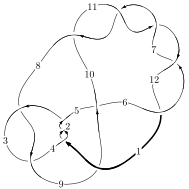
\includegraphics[width=112pt]{../../../GIT/diagram.site/Diagrams/png/1643_12a_0842.png}\\
\ \ \ A knot diagram\footnotemark}&
\allowdisplaybreaks
\textbf{Linearized knot diagam} \\
\cline{2-2}
 &
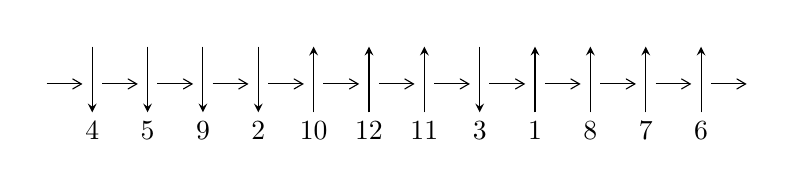
\begin{tikzpicture}[x=20pt, y=17pt]
	% nodes
	\node (C0) at (0, 0) {};
	\node (C1) at (1, 0) {};
	\node (C1U) at (1, +1) {};
	\node (C1D) at (1, -1) {4};

	\node (C2) at (2, 0) {};
	\node (C2U) at (2, +1) {};
	\node (C2D) at (2, -1) {5};

	\node (C3) at (3, 0) {};
	\node (C3U) at (3, +1) {};
	\node (C3D) at (3, -1) {9};

	\node (C4) at (4, 0) {};
	\node (C4U) at (4, +1) {};
	\node (C4D) at (4, -1) {2};

	\node (C5) at (5, 0) {};
	\node (C5U) at (5, +1) {};
	\node (C5D) at (5, -1) {10};

	\node (C6) at (6, 0) {};
	\node (C6U) at (6, +1) {};
	\node (C6D) at (6, -1) {12};

	\node (C7) at (7, 0) {};
	\node (C7U) at (7, +1) {};
	\node (C7D) at (7, -1) {11};

	\node (C8) at (8, 0) {};
	\node (C8U) at (8, +1) {};
	\node (C8D) at (8, -1) {3};

	\node (C9) at (9, 0) {};
	\node (C9U) at (9, +1) {};
	\node (C9D) at (9, -1) {1};

	\node (C10) at (10, 0) {};
	\node (C10U) at (10, +1) {};
	\node (C10D) at (10, -1) {8};

	\node (C11) at (11, 0) {};
	\node (C11U) at (11, +1) {};
	\node (C11D) at (11, -1) {7};

	\node (C12) at (12, 0) {};
	\node (C12U) at (12, +1) {};
	\node (C12D) at (12, -1) {6};
	\node (C13) at (13, 0) {};

	% arrows
	\draw[->,>={angle 60}]
	(C0) edge (C1) (C1) edge (C2) (C2) edge (C3) (C3) edge (C4) (C4) edge (C5) (C5) edge (C6) (C6) edge (C7) (C7) edge (C8) (C8) edge (C9) (C9) edge (C10) (C10) edge (C11) (C11) edge (C12) (C12) edge (C13) ;	\draw[->,>=stealth]
	(C1U) edge (C1D) (C2U) edge (C2D) (C3U) edge (C3D) (C4U) edge (C4D) (C5D) edge (C5U) (C6D) edge (C6U) (C7D) edge (C7U) (C8U) edge (C8D) (C9D) edge (C9U) (C10D) edge (C10U) (C11D) edge (C11U) (C12D) edge (C12U) ;
	\end{tikzpicture} \\
\hhline{~~} \\& 
\textbf{Solving Sequence} \\ \cline{2-2} 
 &
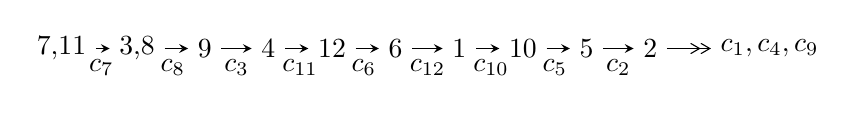
\begin{tikzpicture}[x=23pt, y=7pt]
	% node
	\node (A0) at (-1/8, 0) {7,11};
	\node (A1) at (17/16, 0) {3,8};
	\node (A2) at (17/8, 0) {9};
	\node (A3) at (25/8, 0) {4};
	\node (A4) at (33/8, 0) {12};
	\node (A5) at (41/8, 0) {6};
	\node (A6) at (49/8, 0) {1};
	\node (A7) at (57/8, 0) {10};
	\node (A8) at (65/8, 0) {5};
	\node (A9) at (73/8, 0) {2};
	\node (C1) at (1/2, -1) {$c_{7}$};
	\node (C2) at (13/8, -1) {$c_{8}$};
	\node (C3) at (21/8, -1) {$c_{3}$};
	\node (C4) at (29/8, -1) {$c_{11}$};
	\node (C5) at (37/8, -1) {$c_{6}$};
	\node (C6) at (45/8, -1) {$c_{12}$};
	\node (C7) at (53/8, -1) {$c_{10}$};
	\node (C8) at (61/8, -1) {$c_{5}$};
	\node (C9) at (69/8, -1) {$c_{2}$};
	\node (A10) at (11, 0) {$c_{1},c_{4},c_{9}$};

	% edge
	\draw[->,>=stealth]	
	(A0) edge (A1) (A1) edge (A2) (A2) edge (A3) (A3) edge (A4) (A4) edge (A5) (A5) edge (A6) (A6) edge (A7) (A7) edge (A8) (A8) edge (A9) ;
	\draw[->>,>={angle 60}]	
	(A9) edge (A10);
\end{tikzpicture} \\ 

\end{tabular} \\

\footnotetext{
The image of knot diagram is generated by the software ``\textbf{Draw programme}" developed by Andrew Bartholomew(\url{http://www.layer8.co.uk/maths/draw/index.htm\#Running-draw}), where we modified some parts for our purpose(\url{https://github.com/CATsTAILs/LinksPainter}).
}\phantom \\ \newline 
\centering \textbf{Ideals for irreducible components\footnotemark of $X_{\text{par}}$} 
 
\begin{align*}
I^u_{1}&=\langle 
2 u^{48}-3 u^{47}+\cdots+b-1,\;u^{49}+32 u^{47}+\cdots+a+2,\;u^{50}-2 u^{49}+\cdots+6 u-1\rangle \\
I^u_{2}&=\langle 
u^3+u^2+b+2 u+1,\;- u^4-3 u^2+a-1,\;u^5+u^4+4 u^3+3 u^2+3 u+1\rangle \\
\\
\end{align*}
\raggedright * 2 irreducible components of $\dim_{\mathbb{C}}=0$, with total 55 representations.\\
\footnotetext{All coefficients of polynomials are rational numbers. But the coefficients are sometimes approximated in decimal forms when there is not enough margin.}
\newpage
\renewcommand{\arraystretch}{1}
\centering \section*{I. $I^u_{1}= \langle 2 u^{48}-3 u^{47}+\cdots+b-1,\;u^{49}+32 u^{47}+\cdots+a+2,\;u^{50}-2 u^{49}+\cdots+6 u-1 \rangle$}
\flushleft \textbf{(i) Arc colorings}\\
\begin{tabular}{m{7pt} m{180pt} m{7pt} m{180pt} }
\flushright $a_{7}=$&$\begin{pmatrix}1\\0\end{pmatrix}$ \\
\flushright $a_{11}=$&$\begin{pmatrix}0\\u\end{pmatrix}$ \\
\flushright $a_{3}=$&$\begin{pmatrix}- u^{49}-32 u^{47}+\cdots-3 u-2\\-2 u^{48}+3 u^{47}+\cdots-4 u+1\end{pmatrix}$ \\
\flushright $a_{8}=$&$\begin{pmatrix}1\\- u^2\end{pmatrix}$ \\
\flushright $a_{9}=$&$\begin{pmatrix}- u^9-6 u^7-11 u^5-6 u^3- u\\- u^9-5 u^7-7 u^5-2 u^3+u\end{pmatrix}$ \\
\flushright $a_{4}=$&$\begin{pmatrix}- u^{49}+2 u^{48}+\cdots+2 u-3\\u^{47}-2 u^{46}+\cdots-3 u+1\end{pmatrix}$ \\
\flushright $a_{12}=$&$\begin{pmatrix}u\\u\end{pmatrix}$ \\
\flushright $a_{6}=$&$\begin{pmatrix}u^2+1\\u^2\end{pmatrix}$ \\
\flushright $a_{1}=$&$\begin{pmatrix}u^3+2 u\\u^3+u\end{pmatrix}$ \\
\flushright $a_{10}=$&$\begin{pmatrix}- u\\u^3+u\end{pmatrix}$ \\
\flushright $a_{5}=$&$\begin{pmatrix}- u^6-3 u^4+1\\u^8+4 u^6+4 u^4+2 u^2\end{pmatrix}$ \\
\flushright $a_{2}=$&$\begin{pmatrix}- u^{49}+u^{48}+\cdots+u-2\\- u^{48}+2 u^{47}+\cdots-3 u+1\end{pmatrix}$\\&\end{tabular}
\flushleft \textbf{(ii) Obstruction class $= -1$}\\~\\
\flushleft \textbf{(iii) Cusp Shapes $= - u^{49}+2 u^{48}+\cdots-3 u-10$}\\~\\
\newpage\renewcommand{\arraystretch}{1}
\flushleft \textbf{(iv) u-Polynomials at the component}\newline \\
\begin{tabular}{m{50pt}|m{274pt}}
Crossings & \hspace{64pt}u-Polynomials at each crossing \\
\hline $$\begin{aligned}c_{1},c_{2},c_{4}\end{aligned}$$&$\begin{aligned}
&u^{50}-6 u^{49}+\cdots+4 u-1
\end{aligned}$\\
\hline $$\begin{aligned}c_{3},c_{8}\end{aligned}$$&$\begin{aligned}
&u^{50}+u^{49}+\cdots+64 u+32
\end{aligned}$\\
\hline $$\begin{aligned}c_{5}\end{aligned}$$&$\begin{aligned}
&u^{50}+2 u^{49}+\cdots-3538 u-1049
\end{aligned}$\\
\hline $$\begin{aligned}c_{6},c_{7},c_{10}\\c_{11},c_{12}\end{aligned}$$&$\begin{aligned}
&u^{50}+2 u^{49}+\cdots-6 u-1
\end{aligned}$\\
\hline $$\begin{aligned}c_{9}\end{aligned}$$&$\begin{aligned}
&u^{50}-6 u^{49}+\cdots-2094 u+279
\end{aligned}$\\
\hline
\end{tabular}\\~\\
\newpage\renewcommand{\arraystretch}{1}
\flushleft \textbf{(v) Riley Polynomials at the component}\newline \\
\begin{tabular}{m{50pt}|m{274pt}}
Crossings & \hspace{64pt}Riley Polynomials at each crossing \\
\hline $$\begin{aligned}c_{1},c_{2},c_{4}\end{aligned}$$&$\begin{aligned}
&y^{50}-50 y^{49}+\cdots+16 y+1
\end{aligned}$\\
\hline $$\begin{aligned}c_{3},c_{8}\end{aligned}$$&$\begin{aligned}
&y^{50}-33 y^{49}+\cdots-7680 y+1024
\end{aligned}$\\
\hline $$\begin{aligned}c_{5}\end{aligned}$$&$\begin{aligned}
&y^{50}+18 y^{49}+\cdots-9892846 y+1100401
\end{aligned}$\\
\hline $$\begin{aligned}c_{6},c_{7},c_{10}\\c_{11},c_{12}\end{aligned}$$&$\begin{aligned}
&y^{50}+66 y^{49}+\cdots-22 y+1
\end{aligned}$\\
\hline $$\begin{aligned}c_{9}\end{aligned}$$&$\begin{aligned}
&y^{50}+30 y^{49}+\cdots-3350862 y+77841
\end{aligned}$\\
\hline
\end{tabular}\\~\\
\newpage\flushleft \textbf{(vi) Complex Volumes and Cusp Shapes}
$$\begin{array}{c|c|c}  
\text{Solutions to }I^u_{1}& \I (\text{vol} + \sqrt{-1}CS) & \text{Cusp shape}\\
 \hline 
\begin{aligned}
u &= -0.241502 + 0.933682 I \\
a &= \phantom{-}0.521403 + 0.320826 I \\
b &= \phantom{-}0.450327 - 0.085914 I\end{aligned}
 & -2.13050 - 2.69655 I & \phantom{-}0.94523 + 4.45521 I \\ \hline\begin{aligned}
u &= -0.241502 - 0.933682 I \\
a &= \phantom{-}0.521403 - 0.320826 I \\
b &= \phantom{-}0.450327 + 0.085914 I\end{aligned}
 & -2.13050 + 2.69655 I & \phantom{-}0.94523 - 4.45521 I \\ \hline\begin{aligned}
u &= \phantom{-}0.224098 + 1.034240 I \\
a &= \phantom{-}2.13283 + 0.91465 I \\
b &= \phantom{-}1.44365 - 0.08763 I\end{aligned}
 & -5.96928 + 1.26789 I & \phantom{-0.000000 } 0 \\ \hline\begin{aligned}
u &= \phantom{-}0.224098 - 1.034240 I \\
a &= \phantom{-}2.13283 - 0.91465 I \\
b &= \phantom{-}1.44365 + 0.08763 I\end{aligned}
 & -5.96928 - 1.26789 I & \phantom{-0.000000 } 0 \\ \hline\begin{aligned}
u &= \phantom{-}0.286948 + 1.018960 I \\
a &= -2.14547 - 1.33637 I \\
b &= -1.63676 - 0.38283 I\end{aligned}
 & -5.25575 + 6.41850 I & \phantom{-0.000000 } 0 \\ \hline\begin{aligned}
u &= \phantom{-}0.286948 - 1.018960 I \\
a &= -2.14547 + 1.33637 I \\
b &= -1.63676 + 0.38283 I\end{aligned}
 & -5.25575 - 6.41850 I & \phantom{-0.000000 } 0 \\ \hline\begin{aligned}
u &= -0.260970 + 1.033400 I \\
a &= -0.934867 - 0.520605 I \\
b &= -0.824900 + 0.201401 I\end{aligned}
 & -7.72397 - 3.91870 I & \phantom{-0.000000 } 0 \\ \hline\begin{aligned}
u &= -0.260970 - 1.033400 I \\
a &= -0.934867 + 0.520605 I \\
b &= -0.824900 - 0.201401 I\end{aligned}
 & -7.72397 + 3.91870 I & \phantom{-0.000000 } 0 \\ \hline\begin{aligned}
u &= \phantom{-}0.331404 + 1.033160 I \\
a &= \phantom{-}1.97777 + 1.46824 I \\
b &= \phantom{-}1.50104 + 0.67230 I\end{aligned}
 & -11.6778 + 10.5158 I & \phantom{-0.000000 } 0 \\ \hline\begin{aligned}
u &= \phantom{-}0.331404 - 1.033160 I \\
a &= \phantom{-}1.97777 - 1.46824 I \\
b &= \phantom{-}1.50104 - 0.67230 I\end{aligned}
 & -11.6778 - 10.5158 I & \phantom{-0.000000 } 0\\
 \hline 
 \end{array}$$\newpage$$\begin{array}{c|c|c}  
\text{Solutions to }I^u_{1}& \I (\text{vol} + \sqrt{-1}CS) & \text{Cusp shape}\\
 \hline 
\begin{aligned}
u &= -0.356837 + 0.800466 I \\
a &= \phantom{-}0.088289 - 1.106300 I \\
b &= -0.427389 - 0.642251 I\end{aligned}
 & -5.40920 - 3.17023 I & -6.24629 + 4.79557 I \\ \hline\begin{aligned}
u &= -0.356837 - 0.800466 I \\
a &= \phantom{-}0.088289 + 1.106300 I \\
b &= -0.427389 + 0.642251 I\end{aligned}
 & -5.40920 + 3.17023 I & -6.24629 - 4.79557 I \\ \hline\begin{aligned}
u &= \phantom{-}0.192571 + 1.121550 I \\
a &= -1.64217 - 0.83532 I \\
b &= -0.897289 + 0.086810 I\end{aligned}
 & -13.33180 - 1.81050 I & \phantom{-0.000000 } 0 \\ \hline\begin{aligned}
u &= \phantom{-}0.192571 - 1.121550 I \\
a &= -1.64217 + 0.83532 I \\
b &= -0.897289 - 0.086810 I\end{aligned}
 & -13.33180 + 1.81050 I & \phantom{-0.000000 } 0 \\ \hline\begin{aligned}
u &= \phantom{-}0.063290 + 0.852837 I \\
a &= \phantom{-}1.48467 - 0.76548 I \\
b &= \phantom{-}0.436324 - 1.223550 I\end{aligned}
 & -3.68295 + 0.97203 I & -6.12133 + 0.71322 I \\ \hline\begin{aligned}
u &= \phantom{-}0.063290 - 0.852837 I \\
a &= \phantom{-}1.48467 + 0.76548 I \\
b &= \phantom{-}0.436324 + 1.223550 I\end{aligned}
 & -3.68295 - 0.97203 I & -6.12133 - 0.71322 I \\ \hline\begin{aligned}
u &= -0.168142 + 0.755805 I \\
a &= -0.665021 + 0.730022 I \\
b &= \phantom{-}0.037081 + 0.681718 I\end{aligned}
 & -0.89055 - 1.70206 I & \phantom{-}0.92164 + 5.53470 I \\ \hline\begin{aligned}
u &= -0.168142 - 0.755805 I \\
a &= -0.665021 - 0.730022 I \\
b &= \phantom{-}0.037081 - 0.681718 I\end{aligned}
 & -0.89055 + 1.70206 I & \phantom{-}0.92164 - 5.53470 I \\ \hline\begin{aligned}
u &= \phantom{-}0.473458 + 0.447921 I \\
a &= -0.132112 + 0.553984 I \\
b &= -1.136560 - 0.435330 I\end{aligned}
 & -8.33174 - 4.01114 I & -4.65273 - 0.13384 I \\ \hline\begin{aligned}
u &= \phantom{-}0.473458 - 0.447921 I \\
a &= -0.132112 - 0.553984 I \\
b &= -1.136560 + 0.435330 I\end{aligned}
 & -8.33174 + 4.01114 I & -4.65273 + 0.13384 I\\
 \hline 
 \end{array}$$\newpage$$\begin{array}{c|c|c}  
\text{Solutions to }I^u_{1}& \I (\text{vol} + \sqrt{-1}CS) & \text{Cusp shape}\\
 \hline 
\begin{aligned}
u &= \phantom{-}0.567490 + 0.251389 I \\
a &= -0.16497 - 1.91694 I \\
b &= \phantom{-}0.866292 - 0.017602 I\end{aligned}
 & -7.69762 + 7.46027 I & -2.75082 - 6.53209 I \\ \hline\begin{aligned}
u &= \phantom{-}0.567490 - 0.251389 I \\
a &= -0.16497 + 1.91694 I \\
b &= \phantom{-}0.866292 + 0.017602 I\end{aligned}
 & -7.69762 - 7.46027 I & -2.75082 + 6.53209 I \\ \hline\begin{aligned}
u &= -0.575142\phantom{ +0.000000I} \\
a &= \phantom{-}1.40804\phantom{ +0.000000I} \\
b &= \phantom{-}0.628444\phantom{ +0.000000I}\end{aligned}
 & -2.98861\phantom{ +0.000000I} & -1.42680\phantom{ +0.000000I} \\ \hline\begin{aligned}
u &= \phantom{-}0.494918 + 0.244793 I \\
a &= \phantom{-}0.62020 + 1.67737 I \\
b &= -0.808413 - 0.141535 I\end{aligned}
 & -1.34530 + 3.74735 I & -0.07289 - 7.40976 I \\ \hline\begin{aligned}
u &= \phantom{-}0.494918 - 0.244793 I \\
a &= \phantom{-}0.62020 - 1.67737 I \\
b &= -0.808413 + 0.141535 I\end{aligned}
 & -1.34530 - 3.74735 I & -0.07289 + 7.40976 I \\ \hline\begin{aligned}
u &= -0.457183 + 0.286466 I \\
a &= \phantom{-}1.10902 - 1.15755 I \\
b &= \phantom{-}0.256004 - 0.666486 I\end{aligned}
 & -3.64157 - 1.46138 I & -1.93416 + 4.24780 I \\ \hline\begin{aligned}
u &= -0.457183 - 0.286466 I \\
a &= \phantom{-}1.10902 + 1.15755 I \\
b &= \phantom{-}0.256004 + 0.666486 I\end{aligned}
 & -3.64157 + 1.46138 I & -1.93416 - 4.24780 I \\ \hline\begin{aligned}
u &= \phantom{-}0.394100 + 0.341086 I \\
a &= -0.674932 - 0.693216 I \\
b &= \phantom{-}0.860383 + 0.378414 I\end{aligned}
 & -1.76393 - 0.83267 I & -2.37494 - 0.63227 I \\ \hline\begin{aligned}
u &= \phantom{-}0.394100 - 0.341086 I \\
a &= -0.674932 + 0.693216 I \\
b &= \phantom{-}0.860383 - 0.378414 I\end{aligned}
 & -1.76393 + 0.83267 I & -2.37494 + 0.63227 I \\ \hline\begin{aligned}
u &= -0.425320 + 0.091898 I \\
a &= -0.743778 + 0.682945 I \\
b &= -0.228701 + 0.291111 I\end{aligned}
 & \phantom{-}1.018590 - 0.418472 I & \phantom{-}8.77405 + 2.00502 I\\
 \hline 
 \end{array}$$\newpage$$\begin{array}{c|c|c}  
\text{Solutions to }I^u_{1}& \I (\text{vol} + \sqrt{-1}CS) & \text{Cusp shape}\\
 \hline 
\begin{aligned}
u &= -0.425320 - 0.091898 I \\
a &= -0.743778 - 0.682945 I \\
b &= -0.228701 - 0.291111 I\end{aligned}
 & \phantom{-}1.018590 + 0.418472 I & \phantom{-}8.77405 - 2.00502 I \\ \hline\begin{aligned}
u &= -0.06654 + 1.65140 I \\
a &= -0.502139 + 0.521102 I \\
b &= -0.41662 + 1.56312 I\end{aligned}
 & -13.8965 - 4.6518 I & \phantom{-0.000000 } 0 \\ \hline\begin{aligned}
u &= -0.06654 - 1.65140 I \\
a &= -0.502139 - 0.521102 I \\
b &= -0.41662 - 1.56312 I\end{aligned}
 & -13.8965 + 4.6518 I & \phantom{-0.000000 } 0 \\ \hline\begin{aligned}
u &= -0.02318 + 1.67172 I \\
a &= \phantom{-}0.751552 - 0.327513 I \\
b &= \phantom{-}1.43271 - 1.45403 I\end{aligned}
 & -9.55272 - 2.27084 I & \phantom{-0.000000 } 0 \\ \hline\begin{aligned}
u &= -0.02318 - 1.67172 I \\
a &= \phantom{-}0.751552 + 0.327513 I \\
b &= \phantom{-}1.43271 + 1.45403 I\end{aligned}
 & -9.55272 + 2.27084 I & \phantom{-0.000000 } 0 \\ \hline\begin{aligned}
u &= \phantom{-}0.01016 + 1.69219 I \\
a &= -1.348610 + 0.394636 I \\
b &= -3.15245 + 1.83141 I\end{aligned}
 & -12.79330 + 1.21246 I & \phantom{-0.000000 } 0 \\ \hline\begin{aligned}
u &= \phantom{-}0.01016 - 1.69219 I \\
a &= -1.348610 - 0.394636 I \\
b &= -3.15245 - 1.83141 I\end{aligned}
 & -12.79330 - 1.21246 I & \phantom{-0.000000 } 0 \\ \hline\begin{aligned}
u &= -0.06031 + 1.70334 I \\
a &= -0.294056 - 0.407025 I \\
b &= -0.897079 - 0.594388 I\end{aligned}
 & -11.49630 - 3.87362 I & \phantom{-0.000000 } 0 \\ \hline\begin{aligned}
u &= -0.06031 - 1.70334 I \\
a &= -0.294056 + 0.407025 I \\
b &= -0.897079 + 0.594388 I\end{aligned}
 & -11.49630 + 3.87362 I & \phantom{-0.000000 } 0 \\ \hline\begin{aligned}
u &= \phantom{-}0.07470 + 1.72501 I \\
a &= \phantom{-}2.31285 + 0.82742 I \\
b &= \phantom{-}5.82899 + 2.24727 I\end{aligned}
 & -15.0169 + 7.8885 I & \phantom{-0.000000 } 0\\
 \hline 
 \end{array}$$\newpage$$\begin{array}{c|c|c}  
\text{Solutions to }I^u_{1}& \I (\text{vol} + \sqrt{-1}CS) & \text{Cusp shape}\\
 \hline 
\begin{aligned}
u &= \phantom{-}0.07470 - 1.72501 I \\
a &= \phantom{-}2.31285 - 0.82742 I \\
b &= \phantom{-}5.82899 - 2.24727 I\end{aligned}
 & -15.0169 - 7.8885 I & \phantom{-0.000000 } 0 \\ \hline\begin{aligned}
u &= \phantom{-}0.05873 + 1.72830 I \\
a &= -2.35182 - 0.61319 I \\
b &= -5.90142 - 1.36111 I\end{aligned}
 & -15.8315 + 2.4299 I & \phantom{-0.000000 } 0 \\ \hline\begin{aligned}
u &= \phantom{-}0.05873 - 1.72830 I \\
a &= -2.35182 + 0.61319 I \\
b &= -5.90142 + 1.36111 I\end{aligned}
 & -15.8315 - 2.4299 I & \phantom{-0.000000 } 0 \\ \hline\begin{aligned}
u &= -0.06774 + 1.72877 I \\
a &= \phantom{-}0.495071 + 0.829683 I \\
b &= \phantom{-}1.48829 + 1.29304 I\end{aligned}
 & -17.5722 - 5.2629 I & \phantom{-0.000000 } 0 \\ \hline\begin{aligned}
u &= -0.06774 - 1.72877 I \\
a &= \phantom{-}0.495071 - 0.829683 I \\
b &= \phantom{-}1.48829 - 1.29304 I\end{aligned}
 & -17.5722 + 5.2629 I & \phantom{-0.000000 } 0 \\ \hline\begin{aligned}
u &= \phantom{-}0.08767 + 1.72869 I \\
a &= -2.17648 - 0.82127 I \\
b &= -5.31736 - 2.45060 I\end{aligned}
 & \phantom{-}17.9962 + 12.2318 I & \phantom{-0.000000 } 0 \\ \hline\begin{aligned}
u &= \phantom{-}0.08767 - 1.72869 I \\
a &= -2.17648 + 0.82127 I \\
b &= -5.31736 + 2.45060 I\end{aligned}
 & \phantom{-}17.9962 - 12.2318 I & \phantom{-0.000000 } 0 \\ \hline\begin{aligned}
u &= \phantom{-}0.04560 + 1.74772 I \\
a &= \phantom{-}2.09491 + 0.62616 I \\
b &= \phantom{-}4.94329 + 1.19565 I\end{aligned}
 & \phantom{-}15.8438 - 0.8328 I & \phantom{-0.000000 } 0 \\ \hline\begin{aligned}
u &= \phantom{-}0.04560 - 1.74772 I \\
a &= \phantom{-}2.09491 - 0.62616 I \\
b &= \phantom{-}4.94329 - 1.19565 I\end{aligned}
 & \phantom{-}15.8438 + 0.8328 I & \phantom{-0.000000 } 0 \\ \hline\begin{aligned}
u &= \phantom{-}0.220298\phantom{ +0.000000I} \\
a &= -3.03230\phantom{ +0.000000I} \\
b &= \phantom{-}0.572682\phantom{ +0.000000I}\end{aligned}
 & -1.27955\phantom{ +0.000000I} & -10.7800\phantom{ +0.000000I}\\
 \hline 
 \end{array}$$\newpage\newpage\renewcommand{\arraystretch}{1}
\centering \section*{II. $I^u_{2}= \langle u^3+u^2+b+2 u+1,\;- u^4-3 u^2+a-1,\;u^5+u^4+4 u^3+3 u^2+3 u+1 \rangle$}
\flushleft \textbf{(i) Arc colorings}\\
\begin{tabular}{m{7pt} m{180pt} m{7pt} m{180pt} }
\flushright $a_{7}=$&$\begin{pmatrix}1\\0\end{pmatrix}$ \\
\flushright $a_{11}=$&$\begin{pmatrix}0\\u\end{pmatrix}$ \\
\flushright $a_{3}=$&$\begin{pmatrix}u^4+3 u^2+1\\- u^3- u^2-2 u-1\end{pmatrix}$ \\
\flushright $a_{8}=$&$\begin{pmatrix}1\\- u^2\end{pmatrix}$ \\
\flushright $a_{9}=$&$\begin{pmatrix}1\\- u^2\end{pmatrix}$ \\
\flushright $a_{4}=$&$\begin{pmatrix}u^4+3 u^2+1\\- u^3- u^2-2 u-1\end{pmatrix}$ \\
\flushright $a_{12}=$&$\begin{pmatrix}u\\u\end{pmatrix}$ \\
\flushright $a_{6}=$&$\begin{pmatrix}u^2+1\\u^2\end{pmatrix}$ \\
\flushright $a_{1}=$&$\begin{pmatrix}u^3+2 u\\u^3+u\end{pmatrix}$ \\
\flushright $a_{10}=$&$\begin{pmatrix}- u\\u^3+u\end{pmatrix}$ \\
\flushright $a_{5}=$&$\begin{pmatrix}- u^3-2 u\\- u^3- u\end{pmatrix}$ \\
\flushright $a_{2}=$&$\begin{pmatrix}u^4+u^3+3 u^2+2 u+1\\- u^2- u-1\end{pmatrix}$\\&\end{tabular}
\flushleft \textbf{(ii) Obstruction class $= 1$}\\~\\
\flushleft \textbf{(iii) Cusp Shapes $= 5 u^4+5 u^3+20 u^2+14 u+9$}\\~\\
\newpage\renewcommand{\arraystretch}{1}
\flushleft \textbf{(iv) u-Polynomials at the component}\newline \\
\begin{tabular}{m{50pt}|m{274pt}}
Crossings & \hspace{64pt}u-Polynomials at each crossing \\
\hline $$\begin{aligned}c_{1},c_{2}\end{aligned}$$&$\begin{aligned}
&(u-1)^5
\end{aligned}$\\
\hline $$\begin{aligned}c_{3},c_{8}\end{aligned}$$&$\begin{aligned}
&u^5
\end{aligned}$\\
\hline $$\begin{aligned}c_{4}\end{aligned}$$&$\begin{aligned}
&(u+1)^5
\end{aligned}$\\
\hline $$\begin{aligned}c_{5},c_{9}\end{aligned}$$&$\begin{aligned}
&u^5+u^4- u^2+u+1
\end{aligned}$\\
\hline $$\begin{aligned}c_{6},c_{7}\end{aligned}$$&$\begin{aligned}
&u^5+u^4+4 u^3+3 u^2+3 u+1
\end{aligned}$\\
\hline $$\begin{aligned}c_{10},c_{11},c_{12}\end{aligned}$$&$\begin{aligned}
&u^5- u^4+4 u^3-3 u^2+3 u-1
\end{aligned}$\\
\hline
\end{tabular}\\~\\
\newpage\renewcommand{\arraystretch}{1}
\flushleft \textbf{(v) Riley Polynomials at the component}\newline \\
\begin{tabular}{m{50pt}|m{274pt}}
Crossings & \hspace{64pt}Riley Polynomials at each crossing \\
\hline $$\begin{aligned}c_{1},c_{2},c_{4}\end{aligned}$$&$\begin{aligned}
&(y-1)^5
\end{aligned}$\\
\hline $$\begin{aligned}c_{3},c_{8}\end{aligned}$$&$\begin{aligned}
&y^5
\end{aligned}$\\
\hline $$\begin{aligned}c_{5},c_{9}\end{aligned}$$&$\begin{aligned}
&y^5- y^4+4 y^3-3 y^2+3 y-1
\end{aligned}$\\
\hline $$\begin{aligned}c_{6},c_{7},c_{10}\\c_{11},c_{12}\end{aligned}$$&$\begin{aligned}
&y^5+7 y^4+16 y^3+13 y^2+3 y-1
\end{aligned}$\\
\hline
\end{tabular}\\~\\
\newpage\flushleft \textbf{(vi) Complex Volumes and Cusp Shapes}
$$\begin{array}{c|c|c}  
\text{Solutions to }I^u_{2}& \I (\text{vol} + \sqrt{-1}CS) & \text{Cusp shape}\\
 \hline 
\begin{aligned}
u &= -0.233677 + 0.885557 I \\
a &= -0.827780 - 0.637683 I \\
b &= -0.340036 - 0.807849 I\end{aligned}
 & -3.46474 - 2.21397 I & -4.37343 + 4.39306 I \\ \hline\begin{aligned}
u &= -0.233677 - 0.885557 I \\
a &= -0.827780 + 0.637683 I \\
b &= -0.340036 + 0.807849 I\end{aligned}
 & -3.46474 + 2.21397 I & -4.37343 - 4.39306 I \\ \hline\begin{aligned}
u &= -0.416284\phantom{ +0.000000I} \\
a &= \phantom{-}1.54991\phantom{ +0.000000I} \\
b &= -0.268586\phantom{ +0.000000I}\end{aligned}
 & -0.762751\phantom{ +0.000000I} & \phantom{-}6.42730\phantom{ +0.000000I} \\ \hline\begin{aligned}
u &= -0.05818 + 1.69128 I \\
a &= \phantom{-}0.552827 + 0.534136 I \\
b &= \phantom{-}1.47433 + 1.63485 I\end{aligned}
 & -12.60320 - 3.33174 I & -5.84024 + 1.26157 I \\ \hline\begin{aligned}
u &= -0.05818 - 1.69128 I \\
a &= \phantom{-}0.552827 - 0.534136 I \\
b &= \phantom{-}1.47433 - 1.63485 I\end{aligned}
 & -12.60320 + 3.33174 I & -5.84024 - 1.26157 I\\
 \hline 
 \end{array}$$\newpage
\newpage\renewcommand{\arraystretch}{1}
\centering \section*{ III. u-Polynomials}
\begin{tabular}{m{50pt}|m{274pt}}
Crossings & \hspace{64pt}u-Polynomials at each crossing \\
\hline $$\begin{aligned}c_{1},c_{2}\end{aligned}$$&$\begin{aligned}
&((u-1)^5)(u^{50}-6 u^{49}+\cdots+4 u-1)
\end{aligned}$\\
\hline $$\begin{aligned}c_{3},c_{8}\end{aligned}$$&$\begin{aligned}
&u^5(u^{50}+u^{49}+\cdots+64 u+32)
\end{aligned}$\\
\hline $$\begin{aligned}c_{4}\end{aligned}$$&$\begin{aligned}
&((u+1)^5)(u^{50}-6 u^{49}+\cdots+4 u-1)
\end{aligned}$\\
\hline $$\begin{aligned}c_{5}\end{aligned}$$&$\begin{aligned}
&(u^5+u^4- u^2+u+1)(u^{50}+2 u^{49}+\cdots-3538 u-1049)
\end{aligned}$\\
\hline $$\begin{aligned}c_{6},c_{7}\end{aligned}$$&$\begin{aligned}
&(u^5+u^4+4 u^3+3 u^2+3 u+1)(u^{50}+2 u^{49}+\cdots-6 u-1)
\end{aligned}$\\
\hline $$\begin{aligned}c_{9}\end{aligned}$$&$\begin{aligned}
&(u^5+u^4- u^2+u+1)(u^{50}-6 u^{49}+\cdots-2094 u+279)
\end{aligned}$\\
\hline $$\begin{aligned}c_{10},c_{11},c_{12}\end{aligned}$$&$\begin{aligned}
&(u^5- u^4+4 u^3-3 u^2+3 u-1)(u^{50}+2 u^{49}+\cdots-6 u-1)
\end{aligned}$\\
\hline
\end{tabular}\newpage\renewcommand{\arraystretch}{1}
\centering \section*{ IV. Riley Polynomials}
\begin{tabular}{m{50pt}|m{274pt}}
Crossings & \hspace{64pt}Riley Polynomials at each crossing \\
\hline $$\begin{aligned}c_{1},c_{2},c_{4}\end{aligned}$$&$\begin{aligned}
&((y-1)^5)(y^{50}-50 y^{49}+\cdots+16 y+1)
\end{aligned}$\\
\hline $$\begin{aligned}c_{3},c_{8}\end{aligned}$$&$\begin{aligned}
&y^5(y^{50}-33 y^{49}+\cdots-7680 y+1024)
\end{aligned}$\\
\hline $$\begin{aligned}c_{5}\end{aligned}$$&$\begin{aligned}
&(y^5- y^4+4 y^3-3 y^2+3 y-1)\\
&\cdot(y^{50}+18 y^{49}+\cdots-9892846 y+1100401)
\end{aligned}$\\
\hline $$\begin{aligned}c_{6},c_{7},c_{10}\\c_{11},c_{12}\end{aligned}$$&$\begin{aligned}
&(y^5+7 y^4+16 y^3+13 y^2+3 y-1)(y^{50}+66 y^{49}+\cdots-22 y+1)
\end{aligned}$\\
\hline $$\begin{aligned}c_{9}\end{aligned}$$&$\begin{aligned}
&(y^5- y^4+4 y^3-3 y^2+3 y-1)(y^{50}+30 y^{49}+\cdots-3350862 y+77841)
\end{aligned}$\\
\hline
\end{tabular}
\vskip 2pc
\end{document}